% Project 1, Pattern Recognition, ENEE712, UMBC, Professor Chang
% Author: Bernard Lampe

% Use the IEEE classes
\documentclass[journal]{IEEEtran}

% Packages
\usepackage[cmex10]{amsmath}
\usepackage{url}
\usepackage{cite}
\usepackage{graphicx}
\usepackage{subfig}
\usepackage{float}

% Correct bad hyphenation here
\hyphenation{op-tical net-works semi-conduc-tor}
\DeclareMathOperator*{\argmax}{arg\,max}

% Start document
\begin{document}

% Paper title
\title{Bayesian Classification using Parametric and Non-Parametric Density Estimation Methods}

% Author
\author{Bernard~Lampe,~\IEEEmembership{Member,~IEEE}}

% The paper headers
\markboth{Bayesian Classification using Parametric and Non-Parametric Density Estimation Methods}
{Shell \MakeLowercase{\Lampe}: Bayesian Classification using Parametric and Non-Parametric Density Estimation Methods}

% Make the title area
\maketitle

\begin{abstract}
In this study we demonstrate Bayesian classification using a priori knowledge with maximum likelihood classification and a posteriori knowledge with maximum a posteriori classification. The probabilities used by the classifiers are estimated from a labeled training set using parametric and non-parametric methods during supervised learning. We evaluate the accuracy of the density estimation methods over a range of constraints using the Kullback-Leibler divergence in order to find optimal parameters. Also, we evaluate the effectiveness of the density estimation methods over the same range of constraints using the classification rates. Finally, we assess the performance of the Bayesian classifiers using the different density estimation methods. All data used for the experiments and density estimation were generated via a parametrized Bernoulli distribution (biased coins).
\end{abstract}

% Keywords
\begin{IEEEkeywords}
Bayesian, MLE, Maximum Likelihood Classification, MAP, Maximum APosterior Classification, Parametric, Non-Parametric, Density Estimation, Histogram, Parzen, Gaussian Kernel, K-Nearest Neighbor, Gaussian Fit, Expectation Maximization
\end{IEEEkeywords}

% Introduction with drop letter and first word capitalized.
\section{Introduction}

\IEEEPARstart{T}{he} Bayesian approach to pattern classification will classify new evidence based on the known prior probabilities and class conditional probabilities for each extracted feature of the observation. This is done by choosing the maximum of the a priori or a posteriori probabilities computed for each class. This is known as the maximum likelihood classifier or the maximum a posteriori classifier. The new evidence is a feature vector extracted from the observation which is to be classified. The types of features and feature extraction methods are problem specific and will not be addressed in this study. In the real world, the prior probabilities and the class conditional probabilities for each possible feature are often unknown and must be estimated in advance of classification of new evidence. The prior and class conditional probabilities for each class \(C_k\) are denoted as \(p(C_k)\) and \(p(\vec{x} \vert C_k)\) respectfully.
\par In this study, the unconditional probabilities for each feature \(p(\vec{x})\) and class conditional probabilities \(p(\vec{x}\vert C_k)\) are estimated from a labeled training set of data and the prior probabilities \(p(C_k)\) are known. The training data is a set of feature vectors which have been labeled with the correct class. The estimation of these probabilities is known as supervised learning and can be done in a parametric or non-parametric manner. The parametric methods require the assumption of a parametrized model for the PDF and the parameters for these models can be estimated from the training data. The non-parametric methods do not assume a model and compute the estimate of the PDF directly.
\par The Bayesian decision rule for the Maximum Likelihood Classifier is in equation \ref{eq:mle_decision} and the Maximum Aposteriori Classifier is in equation \ref{eq:map_decision} \cite[p.~17-23]{bishop}.

\begin{equation}
\label{eq:mle_decision}
\text{Decide  } C_k \text{  if  } p(\vec{x} \vert C_k) > p(\vec{x} \vert C_j) \text{    } \forall j \neq k
\end{equation}

\begin{equation}
\label{eq:map_decision}
\text{Decide  } C_k \text{  if  } p(C_k\vert \vec{x}) > p(C_j\vert \vec{x}) \text{    } \forall j \neq k
\end{equation}

\par In this study, the class conditional probabilities \(p(\vec{x} \vert C_k)\) are estimated directly from the training data. The posterior probability is computed from the prior probability \(p(C_k)\), the likelihood of feature \(\vec{x}\) given the class \(C_k\), called the class conditional probability \(p(\vec{x} \vert C_k)\), and the unconditional probability \(p(\vec{x})\). This is accomplished using Bayes rule which turns the prior knowledge into a posteriori knowledge as in equation \ref{eq:posterior_prob} \cite[p.18]{bishop}.

\begin{equation}
\label{eq:posterior_prob}
p(C_k\vert \vec{x}) = \frac{p(\vec{x}\vert C_k)p(C_k)}{p(\vec{x})}
\end{equation}

\par Each of the density estimation methods discussed were evaluated by computing the KL divergence from the known true PDF. The symmetric KL divergence was computed as in equations \ref{eq:kdiv} and \ref{eq:skldiv}.
\begin{equation}
\label{eq:kdiv}
D_{KL}(P,Q) = \sum_{i=1}^{N}{P(i)\log{\frac{P(i)}{Q(i)}}}
\end{equation}

\begin{equation}
\label{eq:skldiv}
D(P,Q) = D_{KL}(P\parallel Q) + D_{KL}(Q\parallel P)
\end{equation}

\par In part two of this study we describe the classifier and the experiment performed to generate new observations. In part three, we explain the training data generation which is used along with a parametric or non-parametric estimation method to estimate the class conditional PDFs which is described in parts four and five. Finally, we evaluate the classification performance of both the MLE and MAP Bayesian classifiers in part six.

% Describe Experiments
\section{Experimental Design}
\par Suppose there is a coin which is modeled by a Bernoulli random variable using parameter \(\theta\) which specifies the probability that the coin will turn up heads on a single flip. If we flip the coin \(d = 100\) times, the outcome is a sequence of heads or tails that will constitute a single experiment or observation. Let this observation be denoted \(\vec{x}_d=(x_1,x_2,\ldots,x_d)^T\) where \(x_i\) is the \(i\)th coin flip. If we perform this experiment multiple times and simply count the number of heads in \(\vec{x}_d\) on each experiment, the results for the number of heads is modeled by a Binomial distribution as in equation \ref{eq:binom}. We denote the number of heads to be simply \(\vec{x}\) with no subscript \(d\) or also \(n_H\).

\begin{equation}
\label{eq:binom}
p(\vec{x} \vert \theta) = \theta^{n_H}(1-\theta)^{d-n_H}
\end{equation}

\par The process of counting the number of heads in a single observation is analogous to the feature extraction step in a pattern recognition system. This is an appropriate feature extraction step because it reduces the dimensionality of the problem by extracting only relevant data needed to classify the bias \(\theta\) from which the observation was generated.

\par The experiment for generating a new observation to be classified proceeds as follows. Assume there are five coins in a box with biases of \(\theta \in \Theta = (0.1, 0.2, 0.3, 0.4, 0.5)\). Randomly select a single coin and flip the coin \(d=100\) times which generates a single observation vector. Then count the number of heads in this observation and denote that as \(\vec{x}\). Then, based on the number of heads, we can classify the observation via the a priori or a posteriori Bayesian approach as follows.

\par Using the a priori approach we can employ the maximum likelihood classifier as in equation \ref{eq:mle_classifier}. These probabilities are computed prior to classification during the training step. During training a PDF is estimated for each class using a parametric or non-parametric estimation method. Then, during classification, we simply look up the value in each of the class conditional PDFs for that particular number of heads and then classify the observation as the class with the highest conditional probability value.

\begin{equation}
\label{eq:mle_classifier}
\text{Choose class   } C_k \text{  as  } \argmax_{C_k}(p(\vec{x}\vert C_k))
\end{equation}

\par Using the a posteriori approach we employ the maximum a posteriori classifier as in equation \ref{eq:map_classifier}. The posterior probabilities for each class are computed using Bayes rule as mentioned in equation \ref{eq:posterior_prob}. For each class, we look up the class conditional PDF value from the estimated PDFs generated during training \(p(\vec{x} \vert C_k)\). Then we convert the known prior probabilities \(p(C_k)\) to the conditional posterior probabilities and then classify the observation as the class with the maximum posterior probability.

\begin{equation}
\label{eq:map_classifier}
\text{Choose class   } C_k \text{  as  } \argmax_{C_k}(p(C_k \vert \vec{x}))
\end{equation}

\section{Training Data Generation  \(\Delta\)}
\par In this study the training data was simulated by flipping a hypothetical coin \(d=100\) times over and over using different biases. The training observations were labeled by the bias \(\theta\) and the bias is used to specify the class \(C_k\).  The data was generated by flipping 5 coins. The biases are in the set \(\Theta = \{0.1, 0.2, 0.3, 0.4, 0.5\}\). The data pool consists of 3000 samples each of 100 flips such that \(\Delta_k = \{\vec{x}_k^j\}_{j=1}^{200k}\) and \(\Delta = \cup_{k=1}^5{\Delta_k}\). Therefore, 200 samples will be from coin \(k=1\) and \(\theta_{k=1} = 0.1\), 400 samples will be from coin \(k=2\) and \(\theta_{k=2} = 0.2\), etc. Therefore, the unbiased coin will make up a third of the samples. The underlying probability density functions (PDF) for each coin for total number of heads when \(d=100\) are plotted in figure \ref{fig:distros_100}.

\begin{figure}
\centering
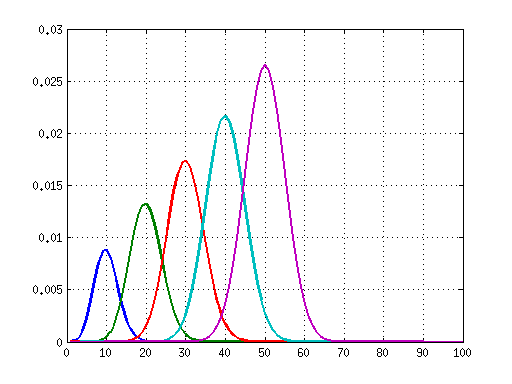
\includegraphics[width=3.3in]{../images/distros_100.png}
\caption{True Class Conditional PDFs of Number of Heads in Training Data, \(p(\vec{x}\vert C_k)\), where \(d=100\)}
\label{fig:distros_100}
\end{figure}

\section{Non-parametric Density Estimation Methods}
\par In this section we describe non-parametric estimation methods used to estimate the probability density functions without assuming a functional form. These methods do require setting constraining parameters on the models, but these parameters are used to determine the amount of smoothing in the final estimate and are set based on problem specific heuristics rather than being estimated from the observations. We consider four of the most common techniques, normalized histogram, Parzen window, Gaussian Kernel and k-nearest neighbors.
\par To evaluate each technique in our specific problem domain, we estimate the unconditional PDFs \(p(\vec{x})\). Then we compute the KL divergence as a measure of how accurate the estimate is to the theoretical binomial distributions. We can use this divergence to select optimal smoothing parameters for each methods. Finally, for each method, we compute the classification rates of the MLE and MAP classifiers to show how performance varies with respect to the smoothing parameters. This also will inform the decision of choosing the optimal values of the smoothing parameters.

\subsection{Density Estimation using Normalized Histograms}
\par The histogram approach to density estimation is very simple. Given the set of feature vectors of size \(N\), divide the feature space into equal bins of size \(h\). Then for the \(k\)th bin, count the number of samples that fall within the bin volume denoted as \(n_k\). The probability of any \(x\) falling in bin \(k\) is approximated by the number of training samples in the bin divided by the number of total samples and the bin volume as shown in equation \ref{eq:histogram_est} \cite{densityhandout}.
\begin{equation}
\label{eq:histogram_est}
p_k(x) \approx \frac{n_k}{N h}
\end{equation}

\par The normalized histogram method was used to estimate the unconditional PDF of the training data \(p(x\vert\Delta)\) and the result is in figure \ref{fig:PDF_Histogram}. The blue bars in the figure show the estimated probabilities, while the red line is the theoretically correct distribution computed from the binomials.

\begin{figure}[h]
\centering
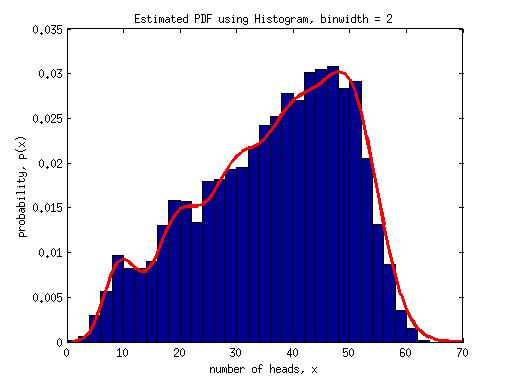
\includegraphics[width=3.3in]{../images/PDF_Histogram.jpg}
\caption{Estimated unconditional PDF of \(p(x)\) using Normalized Histogram with Bin Width Size 2}
\label{fig:PDF_Histogram}
\end{figure}

\par The KL divergence was computed for bin sizes ranging from \(h = 1, 2, \ldots, 10\) and number of samples from \(N = 750, 1500,\ldots, 3750\). As you can see from figure \ref{fig:KL_Histogram}, the KL divergence is smallest when \(h = 2\) and the number of samples is the largest at 3750. This shows that the PDF estimate using the normalized histogram will converge to the theoretical estimated PDF given the correct smoothing parameter \(h\) and a large number of samples.

\begin{figure}[h]
\centering
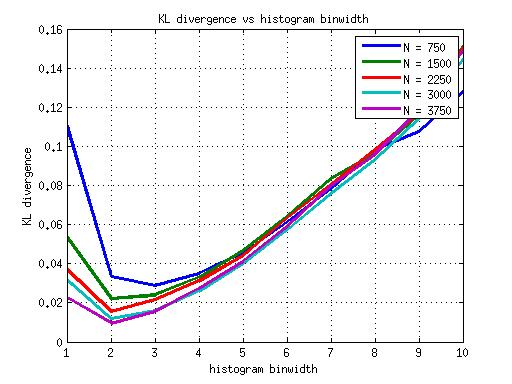
\includegraphics[width=3.3in]{../images/KL_Histogram.jpg}
\caption{KL Divergence versus the Histogram Bin Width for N Samples}
\label{fig:KL_Histogram}
\end{figure}

\par Also the MLE and MAP classification rates were computed as a function of the smoothing parameter using the normalized histogram method. The result is in figure \ref{fig:ClassRate_Histogram}. As you can see, the classification rate decreases as the smoothing parameter increases. As the estimate of the PDF becomes less representative of the true PDF, the error rate goes up.

\begin{figure}[h]
\centering
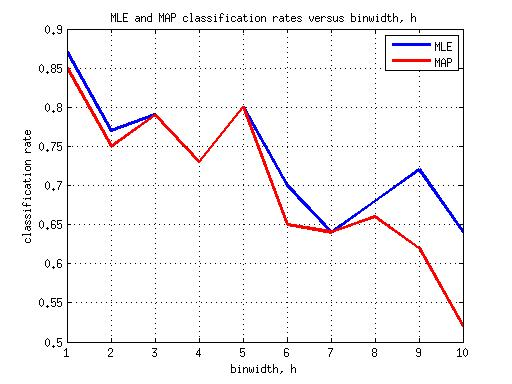
\includegraphics[width=3.3in]{../images/ClassRate_Histogram.jpg}
\caption{MLE and MAP Classification Rates versus Histogram Bin Width}
\label{fig:ClassRate_Histogram}
\end{figure}

\subsection{Density Estimation using Parzen Window}
\par The Parzen window approach to density estimation is related to the histogram approach in that the feature space is divided into discrete regions of uniform size \(h\). However, the Parzen window approach extends to higher dimension feature spaces where as the histogram is most suited only for one dimensional features \cite[p.~164-167]{duda}.
\par Given a set of feature vectors, divide the feature space into hypercube volumes of size \(V\) as in equation \ref{eq:volume}. Also, define a kernel function \(H\) as in equation \ref{eq:kernel} where \(H(\vec{x})\) corresponds to a unit hypercube center at the origin. Thus for all sample vectors in the training set \(\vec{x}^n\), the number of samples \(K\) falling into the hypercube volume around any \(\vec{x}\) is given by equation \ref{eq:kernelsum}. Finally, the estimated probability of any feature vector is given by equation \ref{eq:parzen_est} where the value of \(N\) is the total number of training samples. This method was used to compute the unconditional probabilities of the training data \(p(\vec{x})\) and is show in figure \ref{fig:PDF_Parzen} \cite{densityhandout}.

\begin{equation}
\label{eq:volume}
V = h^d
\end{equation}

\begin{equation}
\label{eq:kernel}
H(\vec{u}) = \left\{
    \begin{array}{lr}
        1 & : \lvert{u_j}\rvert < 1/2\text{, for  } j=1,2,\ldots d \\
        0 & : \text{otherwise}
    \end{array}
    \right.
\end{equation}

\begin{equation}
\label{eq:kernelsum}
K = \sum_{n=1}^{N}{H\left(\frac{\vec{x}^{n}-\vec{x}}{h}\right)}
\end{equation}

\begin{equation}
\label{eq:parzen_est}
p(\vec{x}) \approx \frac{K}{N V} = \frac{1}{N h^d}\sum_{n=1}^{N}{H\left(\frac{\vec{x}^n-\vec{x}}{h}\right)}
\end{equation}

\begin{figure}[h]
\centering
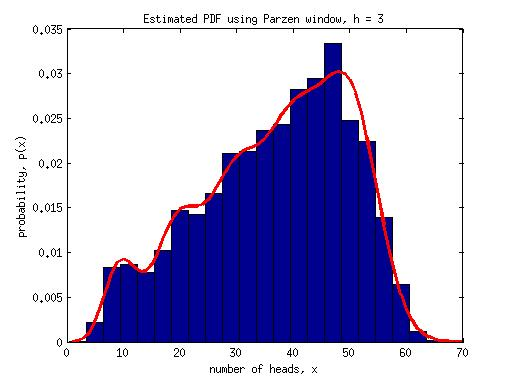
\includegraphics[width=3.3in]{../images/PDF_Parzen.jpg}
\caption{Estimated PDF using Parzen Window with Window Size 3}
\label{fig:PDF_Parzen}
\end{figure}

\par The KL divergence was computed for volume sizes ranging from \(h = 1, 2, \ldots, 10\) and number of samples from \(N = 750, 1500,\ldots, 3750\). As you can see from figure \ref{fig:KL_Parzen}, the KL divergence is smallest when \(h = 3\) and the number of samples is the largest at 3750. This shows that the PDF estimate using the Parzen window method will converge to the theoretical estimated PDF given the correct smoothing parameter \(h\) and a large number of samples.

\begin{figure}[h]
\centering
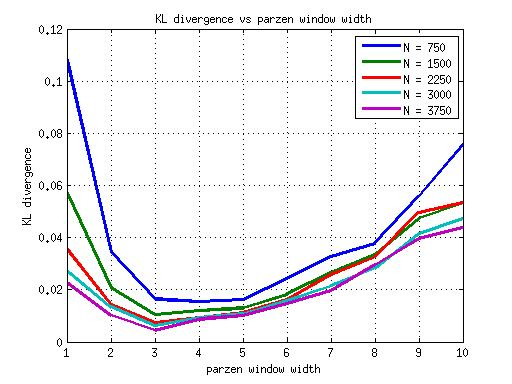
\includegraphics[width=3.3in]{../images/KL_Parzen.jpg}
\caption{KL Divergence versus the Parzen Window Width for N Samples}
\label{fig:KL_Parzen}
\end{figure}

\par Also the MLE and MAP classification rates were computed as a function of the smoothing parameter using the Parzen window method. The result is in figure \ref{fig:ClassRate_Parzen}. As you can see, the classification rate decreases as the smoothing parameter increases. As the estimate of the PDF becomes less representative of the true PDF, the error rate goes up.

\begin{figure}[h]
\centering
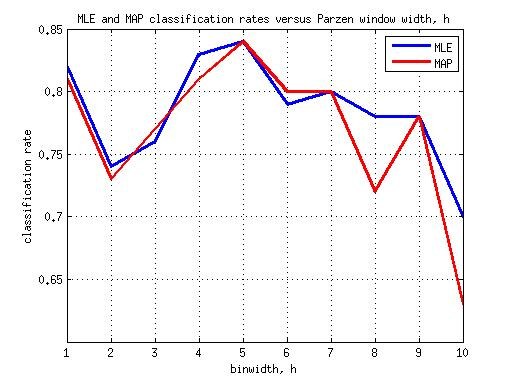
\includegraphics[width=3.3in]{../images/ClassRate_Parzen.jpg}
\caption{MLE and MAP Classification Rates versus Parzen Window Width}
\label{fig:ClassRate_Parzen}
\end{figure}

\subsection{Density Estimation using Gaussian Kernel}
\par The Gaussian kernel approach to density estimation is related to the Parzen window approach in that it can estimate densities of high dimensional feature spaces by dividing the space into regions. The Gaussian kernel approach replaces the Parzen window kernel function \(H\) by a Gaussian distribution thereby spreading the contribution of a single training sample to many hypercubes as a function of distance from the cube centers. The equation for the Gaussian Kernel is \ref{eq:gaussKernel} and is equivalent to a Parzen window where the kernel function is replaces by a hyper dimensional Gaussian function. The unconditional probabilities \(p(\vec{x})\) for the training data were estimated using the Gaussian kernel method and the results are in figure \ref{fig:PDF_GaussianKernel}. Notice that the estimated PDF has a smoother quality but does not lose as many fine details as the histogram or Parzen window methods \cite{densityhandout}.

\begin{equation}
\label{eq:gaussKernel}
p(\vec{x}) \approx \frac{K}{N V} = \frac{1}{N (2\pi h^2)^{d/2}}\sum_{n=1}^{N}{\exp\left(- \frac{\lvert\vec{x}^n-\vec{x}\rvert^2}{2h^2}\right)}
\end{equation}

\begin{figure}[h]
\centering
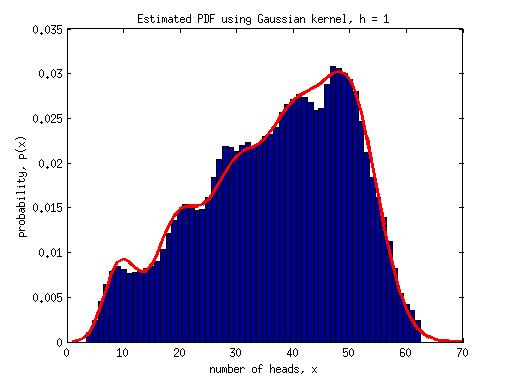
\includegraphics[width=3.3in]{../images/PDF_GaussianKernel.jpg}
\caption{Estimated PDF using Gaussian Kernel with Window Size 1}
\label{fig:PDF_GaussianKernel}
\end{figure}

\par The KL divergence was computed for volume sizes ranging from \(h = 1, 2, \ldots, 10\) and number of samples from \(N = 750, 1500,\ldots, 3750\). As you can see from figure \ref{fig:KL_Parzen}, the KL divergence is smallest when \(h = 1\) or \(h = 2\). This shows that the PDF estimate using the Parzen window method will converge to the theoretical estimated PDF given the correct smoothing parameter. There is a noticeable difference when computing the KL distances using increasing number of samples in that the KL distance is not significantly different between \(750\) samples and \(3750\) samples. This fact suggests that the Gaussian Kernel method is more robust to a smaller number of samples than the histogram or Parzen window methods.

\begin{figure}[h]
\centering
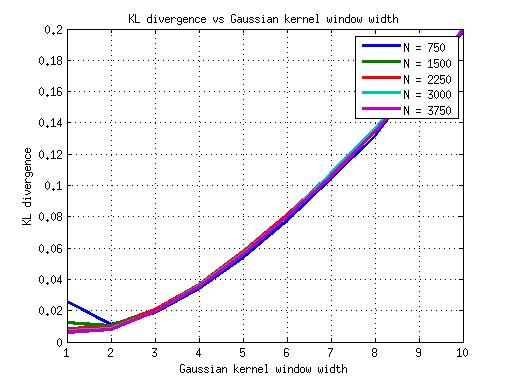
\includegraphics[width=3.3in]{../images/KL_GaussianKernel.jpg}
\caption{KL Divergence versus the Gaussian Kernel Window Width for N Samples}
\label{fig:KL_GaussianKernel}
\end{figure}

\par Also the MLE and MAP classification rates were computed as a function of the smoothing parameter using the Gaussian Kernel method. The result is in figure \ref{fig:ClassRate_GaussianKernel}. As you can see, the classification rate decreases as the volume parameter increases. As the estimate of the PDF becomes less representative of the true PDF, the error rate goes up.

\begin{figure}[h]
\centering
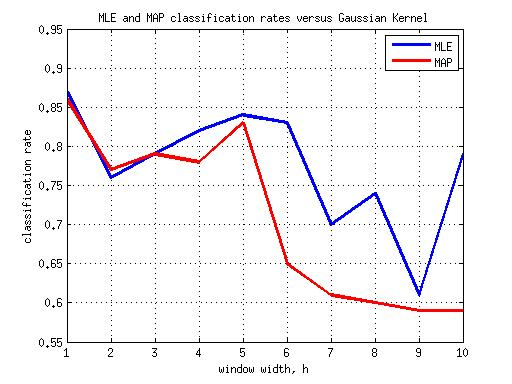
\includegraphics[width=3.3in]{../images/ClassRate_GaussianKernel.jpg}
\caption{MLE and MAP Classification Rates versus Gaussian Kernel Window Width}
\label{fig:ClassRate_GaussianKernel}
\end{figure}

\subsection{Density Estimation using K-Nearest Neighbors}
\par The k-nearest neighbors approach to density estimation is based on the same PDF approximation equation as the prior three methods as in equation \ref{eq:knn_est}. However, with this method, we hold the number of samples \(K\) constant and find the volume in which the \(K\) samples fall. This means the volume can vary. Given the training samples and a fixed \(K\) we vary the volume of the hypercube \(V\) by computing a hypersphere around a sample vector \(\vec{x}\) to include \(K\) points without regard to the class label. This volume is used to estimate the probabilities. The unconditional probabilities of the training set were computed and are show in figure \ref{fig:PDF_KNN} \cite{densityhandout} \cite[p.55-57]{bishop}.

\begin{equation}
\label{eq:knn_est}
p(\vec{x}) \approx \frac{K}{N V}
\end{equation}

\begin{figure}
\centering
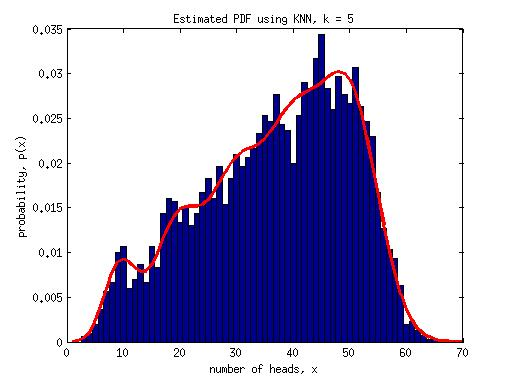
\includegraphics[width=3.3in]{../images/PDF_KNN.jpg}
\caption{Estimated PDF using K-Nearest Neighbors with K = 5}
\label{fig:PDF_KNN}
\end{figure}

\par The KL divergence was computed for K ranging from \(K = 1, 10, \ldots, 100\) and number of samples from \(N = 750, 1500,\ldots, 3750\). As you can see from figure \ref{fig:KL_KNN}, the KL divergence is smallest when \(K = 1\) or \(K = 10\). This shows that the PDF estimate using the KNN is most accurate when the value of \(K\) is small if the number of samples are sufficiently large. Notice, however, when the number of samples becomes sparse, the KNN estimation method requires a larger value of \(K\) to improve the PDF estimate. Also, when the number of samples is small, the KNN method does not perform as well as the histogram, Parzen window or Gaussian kernel methods described above.

\begin{figure}
\centering
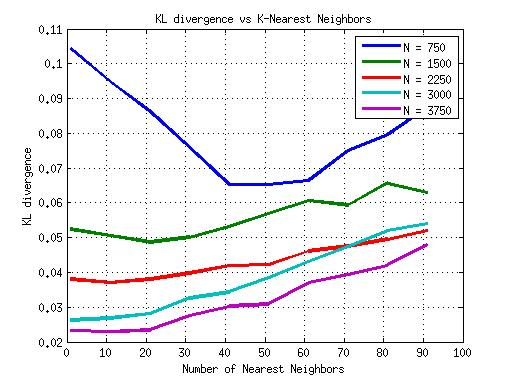
\includegraphics[width=3.3in]{../images/KL_KNN.jpg}
\caption{KL Divergence versus the K for N Samples}
\label{fig:KL_KNN}
\end{figure}

\par Also the MLE and MAP classification rates were computed as a function of the \(K\) using the KNN method. The result is in figure \ref{fig:ClassRate_KNN}. As you can see, the classification rate has a high variance and seems to increase as the the value of \(K\) increases. However, this upward trend is not significant given the variability in the classification rate.

\begin{figure}
\centering
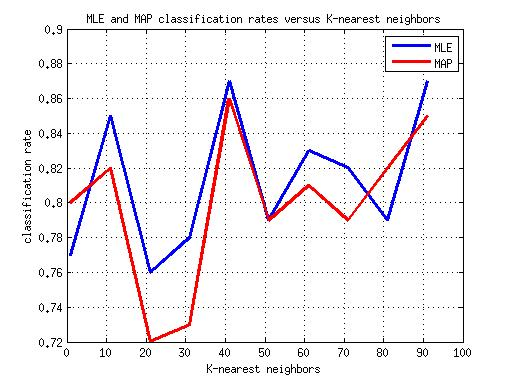
\includegraphics[width=3.3in]{../images/ClassRate_KNN.jpg}
\caption{MLE and MAP Classification Rates versus K using K-Nearest Neighbors}
\label{fig:ClassRate_KNN}
\end{figure}

\section{Parametric Density Estimation Methods}
\par In this section we describe two parametric estimation methods used to estimate probability density functions using an assumed analytical model for which parameters are to be estimated. These parameters are estimated from the training sample. We consider two parametric methods based on the Gaussian distribution. The first is estimating the PDF using a single Gaussian distribution and the second is using a Gaussian mixture model. While the assumption of a particular model without first analyzing the data is a strong one, it is not completely without theoretical basis. The Gaussian is the safest assumption under completely unknown circumstances in that the sum of multiple random variable will tend towards a Gaussian distribution. Also, computing the parameters for a Gaussian is computationally simple and may warrant the tolerance of model error if it does not impact performance negatively.
\par As with the non-parametric methods, we evaluate the PDF estimate using the KL distance and classification performance over a range of model parameters. We use these as performance criteria to determine the best model selection.

\subsection{Density Estimation using a Single Gaussian Model}
\par Using a single Gaussian to estimate the PDF is simple. Given the training data, we estimate the mean and variance of the Gaussian distribution using the best linear unbiased estimators as in equations \ref{eq:mean} and \ref{eq:var}. This method was used to compute the unconditional probabilities \(p(\vec{x})\) as show in figure \ref{fig:PDF_Gaussian}. Notice the fit is not very good and the KL distance was computed as 0.1536 with is high when compared to the any other method described in the paper using 3000 samples in the training set. The classification rate using the Gaussian to compute class conditionals was favorable because a single class is well modeled by a Gaussian. This model is attractive because there are no constraints to optimize and is computationally simple to compute the parameters and a single class conditional distribution may be well modeled by a Gaussian.

\begin{equation}
\label{eq:mean}
\vec{u} = \frac{1}{N}\sum_{n=1}^{N}{\vec{x}}
\end{equation}

\begin{equation}
\label{eq:var}
\sigma^2 = \frac{1}{N-1}\sum_{n=1}^{N}{(\lvert\vec{x} - \vec{u}\rvert)^2}
\end{equation}

\begin{figure}[h]
\centering
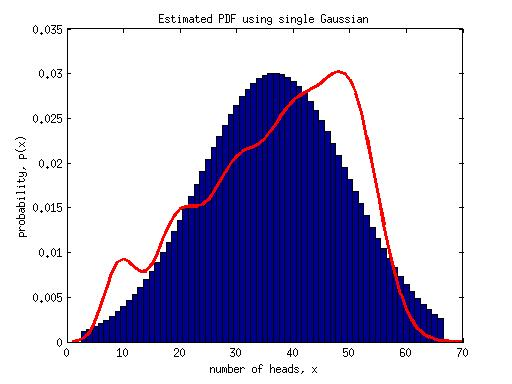
\includegraphics[width=3.3in]{../images/PDF_SingleGaussian.jpg}
\caption{Estimated PDF using a Single Gaussian}
\label{fig:PDF_Gaussian}
\end{figure}

\subsection{Density Estimation using a Gaussian Mixture Model}
\par The Gaussian mixture model approach to PDF estimation assumes that a weighted linear combination of Gaussian will provide an adequate estimate. The parameters for each Gaussian and the weights of the linear combination are computed using the expectation maximization algorithm. The GMM method was used to compute an estimate of the unconditional probabilities of the training set \(p(\vec{x})\) and is show in figure \ref{fig:PDF_GMM_3} using three Gaussians \cite{emhandout}.
\begin{equation}
\label{eq:gaussian}
g(\vec{x}; \vec{\mu_k}, \vec{\sigma_k}) = \frac{1}{(\sqrt{2\pi}\vec{\sigma_k})^D} e^{-\frac{1}{2}\left(\frac{\vec{x}-\vec{\mu_k}}{\vec{\sigma_k}}\right)^2}
\end{equation}

\begin{equation}
\label{eq:mixedpdfs}
p(\vec{x}; \Delta) = \sum_{k=1}^{5}{w_k g(\vec{x}; \vec{\mu_k}, \vec{\sigma_k})}
\end{equation}

\begin{equation}
\label{eq:weight_constrains}
w_k \ge 0 \text{   and   } \sum_{k = 1}^{5}{w_k} = 1
\end{equation}

\par The expectation maximization algorithm is used to iteratively estimate the parameters of the GMM. The parameters are \(\vec{\mu}\), \(\vec{\sigma}\) and \(\vec{w_k}\). The optimization algorithm can be outlined in two steps which run alternately to produce estimates of the parameters which converge. The E-step, estimates the contributions of each Gaussian use the MLE as in equation \ref{eq:estep} \cite{carlo}.
\begin{equation}
\label{eq:estep}
p^{(i)}(k|\vec{x_n}) = \frac{p_k^{(i)}g(\vec{x_n};\mu_k^{(i)},\sigma_k^{(i)})}
{\sum_{m=1}^{5}{p_k^{(i)}g(\vec{x_n};\mu_k^{(i)},\sigma_k^{(i)}})}
\end{equation}

\par The EM algorithm continues with the M-step as in equations \ref{eq:mstep_1}, \ref{eq:mstep_2} and \ref{eq:mstep_3}. These three equations compute the parameters of each of the Gaussian \cite{carlo}.

\begin{equation}
\label{eq:mstep_1}
\mu_k^{(i+1)} = \frac
{\sum_{n=1}^{N}{p^{(i)}(k|\vec{x_n})\vec{x_n}}}
{\sum_{n=1}^{N}{p^{(i)}(k|\vec{x_n})}}
\end{equation}

\begin{equation}
\label{eq:mstep_2}
\sigma_k^{(i+1)} = \sqrt{
\frac{1}{D}
\frac{\sum_{n=1}^N{p^{(i)}(k|\vec{x_n})|\vec{x_n}-\mu_k^{(i+1)}|^2}}
{\sum_{n=1}^N{p^{(i)}(k|\vec{x_n})}}
}
\end{equation}

\begin{equation}
\label{eq:mstep_3}
p_k^{(i+1)} = \frac{1}{N}\sum_{n=1}^N{p^{(i)}(k|\vec{x_n})}
\end{equation}

\begin{figure}
\centering
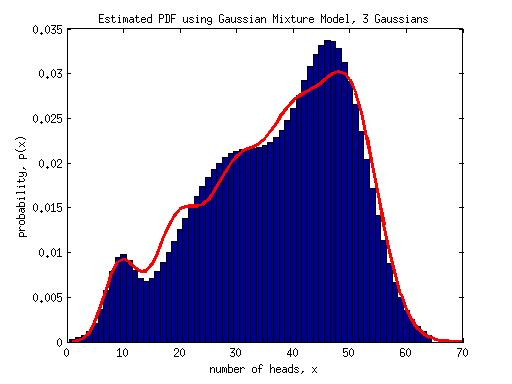
\includegraphics[width=3.3in]{../images/PDF_GMM_3.jpg}
\caption{Estimated PDF using a Gaussian Mixture Model with 3 Gaussians}
\label{fig:PDF_GMM_3}
\end{figure}

\par The KL divergence was computed for the GMM method for \(K\) Gaussians for \(K = 2,\ldots,5\) and for a varying number of samples \(N = 750, 1500, \ldots, 3750\). The KL divergence values are show in figure \ref{fig:KL_GMM}. This shows that 2, 3 or even 4 Gaussians does a good job at estimating the unconditional PDF. However, when using 5 Gaussians the KL divergence increases considerably unless there are a large number of samples. This shows that the GMM method will converge to the true PDF if given an appropriate number of Gaussians and samples.

\begin{figure}
\centering
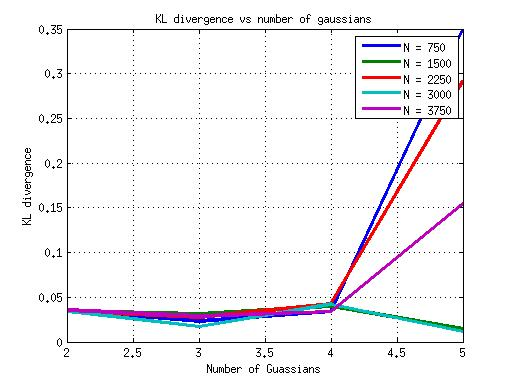
\includegraphics[width=3.3in]{../images/KL_GMM.jpg}
\caption{KL Divergence versus Number of Gaussians for N Samples}
\label{fig:KL_GMM}
\end{figure}

\par Also the classification rates for the GMM method were computed and are shown in figure \ref{fig:ClassRate_GMM}. From the figure, you can see that the classification rate is increasing as the number of Gaussians increases. 

\begin{figure}
\centering
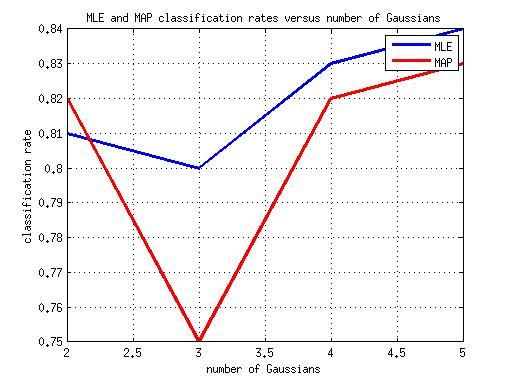
\includegraphics[width=3.3in]{../images/ClassRate_GMM.jpg}
\caption{MLE and MAP Classification Rates versus Number of Gaussians}
\label{fig:ClassRate_GMM}
\end{figure}

\section{Classification}
\par Classification was done using the MLE and MAP classifier rules outlined in the introduction. The class conditional probabilities \(p(\vec{x}\vert C_k)\) were estimated using the four non-parametric and two parametric estimation methods described above. These class conditionals were used directly to estimate the conditional probabilities directly used in the MLE classifier. The class conditionals were then multiplied by the known class prior probabilities \(p(C_k)\) to create the posterior probabilities used in the MAP classifier. The class unconditional probabilities \(p(\vec{x})\) were not needed for classification of a new sample because both rules are a maximum and the unconditional probability of a particular sample will be constant. The important part is the class conditional probabilities.

\subsection{Estimated Class Conditional PDFs}
\par This section shows the estimated class conditional PDFs, \(p(\vec{x}\vert C_k)\), estimated using each of the methods described above. The class conditionals are all show in figures \ref{fig:1}, \ref{fig:2}, \ref{fig:3}, \ref{fig:4}, \ref{fig:5} and \ref{fig:6}.
\begin{figure}[h]
\centering
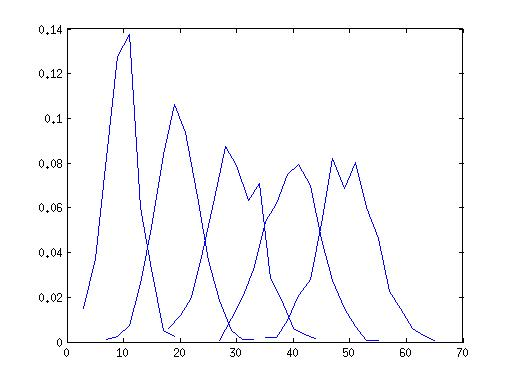
\includegraphics[width=3.3in]{../images/conditional_using_histogram_binwidth2.jpg}
\caption{Class Conditional PDF Estimate using the Non-parametric Histogram Method with 3000 Training Samples and Bin Width 2}
\label{fig:1}
\end{figure}

\begin{figure}
\centering
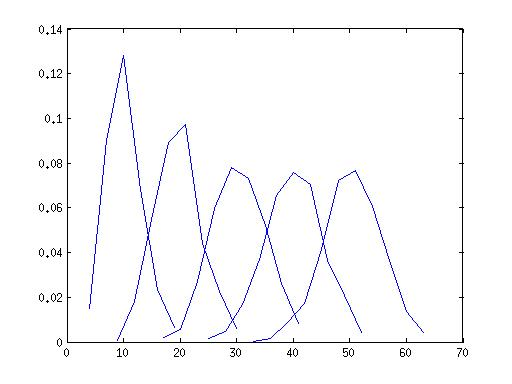
\includegraphics[width=3.3in]{../images/conditional_using_parzen_h3.jpg}
\caption{Class Conditional PDF Estimate using the Non-parametric Parzen Window Method with 3000 Training Samples and Volume Width 3}
\label{fig:2}
\end{figure}

\begin{figure}
\centering
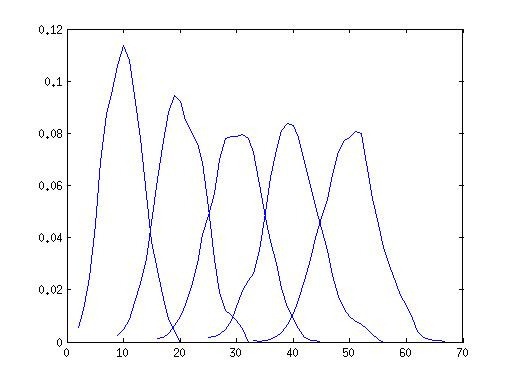
\includegraphics[width=3.3in]{../images/conditional_using_gausKernel_h1.jpg}
\caption{Class Conditional PDF Estimate using the Non-parametric Gaussian Kernel Method with 3000 Training Samples and Kernel Width 1}
\label{fig:3}
\end{figure}

\begin{figure}
\centering
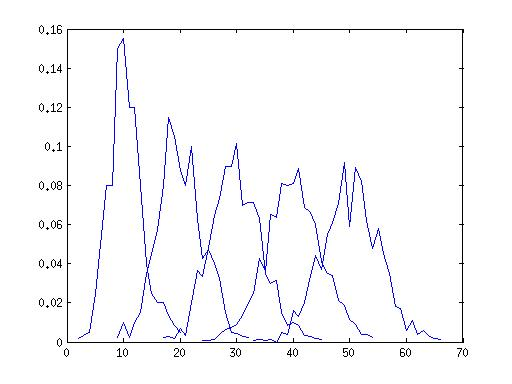
\includegraphics[width=3.3in]{../images/conditional_using_knn_k5.jpg}
\caption{Class Conditional PDF Estimate using the Non-parametric K-Nearest Neighbors Method with 3000 Training Samples and \(K = 5\)}
\label{fig:4}
\end{figure}

\begin{figure}
\centering
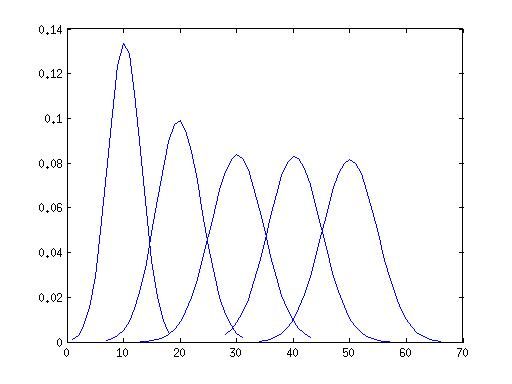
\includegraphics[width=3.3in]{../images/conditional_using_singlegauss.jpg}
\caption{Class Conditional PDF Estimate using the Parametric Single Gaussian Method with 3000 Training Samples}
\label{fig:5}
\end{figure}

\begin{figure}
\centering
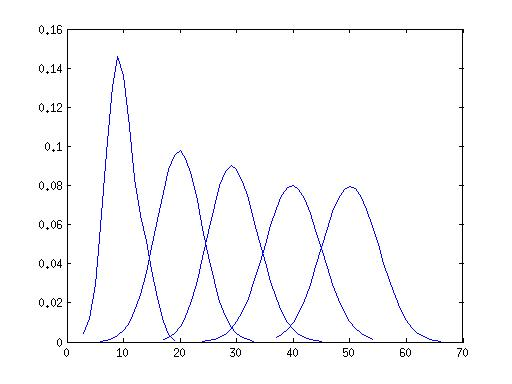
\includegraphics[width=3.3in]{../images/conditional_using_gaussmixture_emalgo.jpg}
\caption{Class Conditional PDF Estimate using the Gaussian Mixture Method with 3000 Training Samples and 2 Gaussians per Class. This does not look appreciably different to the Single Gaussian case because the Gaussians Overlap.}
\label{fig:6}
\end{figure}

\subsection{Classification Rates Per Algorithm}
\par The classification rates of both the MLE and MAP classifiers are show in figures \ref{fig:PDF_ALL_MLE} and \ref{fig:PDF_ALL_MAP}. These classification rates were computed using the entire training sample of 3000 vectors. In addition the constraining parameters used for the non-parametric methods were set to the optimal values as computed using the KL distance. Also the number of Gaussian for the GMM was set using the optimal KL value. In the real world, we would not know these constraining parameters and would have to use a criteria such as AIC or MDL \cite{densityhandout}.


\begin{figure}
\centering
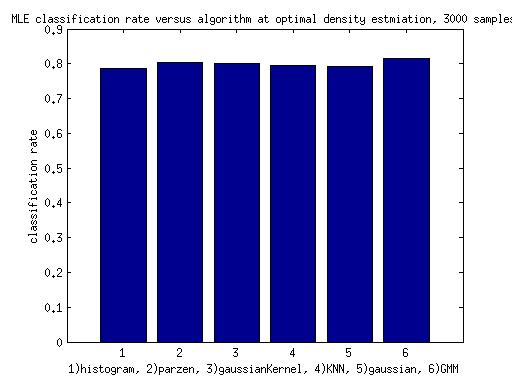
\includegraphics[width=3.3in]{../images/all_algos_mle.jpg}
\caption{MLE Classification Rate of Each Algorithm using Optimal Estimation Parameters and 3000 Samples for Training}
\label{fig:PDF_ALL_MLE}
\end{figure}

\begin{figure}
\centering
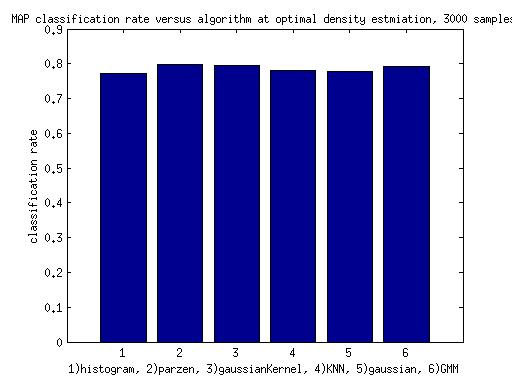
\includegraphics[width=3.3in]{../images/all_algos_map.jpg}
\caption{MAP Classification Rate of Each Algorithm using Optimal Estimation Parameters and 3000 Samples for Training}
\label{fig:PDF_ALL_MAP}
\end{figure}

\section{Conclusion}
\par The evidence revealed by this study suggests that of the non-parametric estimation methods, that Gaussian Kernel method is more robust than the histogram, Parzen window or KNN methods when the number of samples is low. However, the Gaussian kernel method is the most computationally expensive of the non-parametric methods discussed in this study. The histogram and Parzen window methods are a less computationally expensive approximation to the Gaussian kernel. Also, it appears that the K-nearest neighbors method performed the poorest of the non-parametric methods when the number of samples was low as shown by the KL divergence. However, with sufficiently high number of samples, and the right smoothing parameters, each of the methods will converge to the true PDF. Finally, for the histogram, Parzen window and KNN methods, the choice of any of the constraining parameters did not help nearly as much as obtaining more samples. These three methods appear to be limited when the number of samples is small. This does not appear true for the Gaussian kernel method.
\par Also the non-parametric methods are sensitive to their constraints such as bin width, volume width, kernel width and number of neighbors chosen. The determination of these smoothing parameters is problem specific and in the real world, we would not know them ahead of time or be able to compute the KL distance as the true distribution would be unknown to us. As shown by the classification rate, the histogram, Parzen window and Gaussian kernel methods all performed well at the constraints where the KL divergence was the optimal. However the classification rate of the KNN method had a high variance and did not appear to show a discernible trend.
\par Classification rate did not vary considerably when each of the estimation methods was set to the optimal constraining parameters and when using 3000 training samples. The classification rate of the MAP classifier was consistently lower than the MLE classifier because the priors assumed in the training sample were not the priors which were used in the actual experiment. In the training samples we had a prior which was not uniform, but in the experiment we chose a coin at random which implies a uniform prior. The MLE classifier used the correct prior implicitly through the direct estimate of the class conditionals. The MAP used the known, but skewed priors to turn the a priori knowledge into a posteriori knowledge. Using the miss classification rate, we could update the priors and after enough tests could use Bayes rule to arrive at a uniform prior which was the true state of nature of the experiment.


% References section
\nocite{*}
\bibliographystyle{plain}
\bibliography{./references}

% Biography
\begin{IEEEbiographynophoto}{Bernard Lampe}
(M'09) became an IEEE Member (M) in 2009 and received his bachelors of science degree from The University of Michigan in Ann Arbor, Michigan, USA in 2009.
\par Mr. Lampe is also a member of the American Society for Computing Machines (ACM) since 2009.
\end{IEEEbiographynophoto}

% End document
\end{document}

